% ---------------------------------------------------------------------------------------------------------------
% TEMPLATE PARA TRABALHO DE CONCLUSÃO DE CURSO
% Pontifícia Universidade Católica de Minas Gerais - PUC Minas
% Customização da classe abnTeX2 (http://www.abntex.net.br/) para as normas da PUC Minas
% Baseado na classe abnTeX2 da Universidade Federal Tecnológica do Paraná
% Adaptado para seguir as regras de normalização da PUC Minas <http://portal.pucminas.br/biblioteca/>
%
% Autores da customização original: 
%        Diego Marczal
%        Michael Vornes <https://github.com/mvornes>
%
%----------------------------------------------------------------------------------------------------------------
% Codificação: UTF-8
% LaTeX:  abnTeX2          
% ---------------------------------------------------------------------------------------------------------------


% CARREGA CLASSE PERSONALIZADA DA PUC MINAS--------------------------------------------------------------------------
\documentclass[%twoside,                   % Impressão em frente e verso
    	        oneside,                   % Impressão apenas frente
]{configuracoes/pucminas-abntex2}


% INCLUI ARQUIVOS DE CONFIGURAÇÕES-------------------------------------------------------------------------------
% REFERÊNCIAS------------------------------------------------------------------
\usepackage[%
    alf,
    abnt-emphasize=bf,
    bibjustif,
    recuo=0.0cm,
    abnt-url-package=url,       % Utiliza o pacote url
    abnt-refinfo=yes,           % Utiliza o estilo bibliográfico abnt-refinfo
    abnt-etal-cite=3,
    abnt-etal-list=3,
    abnt-thesis-year=final
]{abntex2cite}                  % Configura as citações bibliográficas conforme a norma ABNT

% PACOTES----------------------------------------------------------------------
\usepackage[utf8]{inputenc}                                 % Codificação do documento
\usepackage[T1]{fontenc}                                    % Seleção de código de fonte
\usepackage{booktabs}                                       % Réguas horizontais em tabelas
\usepackage{color, colortbl}                                % Controle das cores
\usepackage{float}                                          % Necessário para tabelas/figuras em ambiente multi-colunas
\usepackage{graphicx}                                       % Inclusão de gráficos e figuras
\usepackage{icomma}                                         % Uso de vírgulas em expressões matemáticas
\usepackage{indentfirst}                                    % Indenta o primeiro parágrafo de cada seção
\usepackage{microtype}                                      % Melhora a justificação do documento
\usepackage{multirow, array}                                % Permite tabelas com múltiplas linhas e colunas
\usepackage{subeqnarray}                                    % Permite subnumeração de equações
\usepackage{lastpage}                                       % Para encontrar última página do documento
\usepackage{verbatim}                                       % Permite apresentar texto tal como escrito no documento, ainda que sejam comandos Latex
\usepackage{amsfonts, amssymb, amsmath}                     % Fontes e símbolos matemáticos
\usepackage[algoruled, portuguese]{algorithm2e}             % Permite escrever algoritmos em português
\usepackage{pslatex}                                        % Usa a fonte Times New Roman
\usepackage[bottom]{footmisc}                               % Mantém as notas de rodapé sempre na mesma posição
\usepackage{ae, aecompl}                                    % Fontes de alta qualidade
\usepackage{latexsym}                                       % Símbolos matemáticos
\usepackage{lscape}                                         % Permite páginas em modo "paisagem"
%\usepackage{picinpar}                                      % Dispor imagens em parágrafos
%\usepackage{scalefnt}                                      % Permite redimensionar tamanho da fonte
%\usepackage{subfig}                                        % Posicionamento de figuras
%\usepackage{upgreek}                                       % Fonte letras gregas

% CONFIGURAÇÕES DE APARÊNCIA DO PDF FINAL--------------------------------------
\makeatletter
\hypersetup{%
    portuguese,
    colorlinks=true,   % true: "links" coloridos; false: "links" em caixas de texto
    linkcolor=blue,    % Define cor dos "links" internos
    citecolor=blue,    % Define cor dos "links" para as referências bibliográficas
    filecolor=blue,    % Define cor dos "links" para arquivos
    urlcolor=blue,     % Define a cor dos "hiperlinks"
    breaklinks=true,
    pdftitle={\@title},
    pdfauthor={\@author},
    pdfkeywords={abnt, latex, abntex, abntex2}
}
\makeatother

% ALTERA O ASPECTO DA COR AZUL--------------------------------------------------
\definecolor{blue}{RGB}{41,5,195}

% REDEFINIÇÃO DE LABELS---------------------------------------------------------
\renewcommand{\algorithmautorefname}{Algoritmo}
\def\equationautorefname~#1\null{Equa\c c\~ao~(#1)\null}

% CRIA ÍNDICE REMISSIVO---------------------------------------------------------
\makeindex

% HIFENIZAÇÃO DE PALAVRAS QUE NÃO ESTÃO NO DICIONÁRIO---------------------------
\hyphenation{%
    qua-dros-cha-ve
    Kat-sa-gge-los
}



% INCLUI ARQUIVOS DO TRABALHO DE CONCLUSÃO DE CURSO (PRÉ-TEXTUAIS, TEXTUAIS, PÓS-TEXTUAIS)-----------------------

% INSERE CAPA E FOLHA DE ROSTO
% CAPA---------------------------------------------------------------------------------------------------

% ORIENTAÇÕES GERAIS-------------------------------------------------------------------------------------
% Caso algum dos campos não se aplique ao seu trabalho, como por exemplo,
% se não houve coorientador, apenas deixe vazio.
% Exemplos: 
% \coorientador{}
% \departamento{}

% DADOS DO TRABALHO--------------------------------------------------------------------------------------
\titulo{Python}
\titleabstract{Python}
\autor{Iyan Lucas Duarte Marques, Samir do Amorim Cambraia, Guilherme Cosso}
\autorcitacao{MARQUES, D. Iyan Lucas, Cambraia, A. Samir, COSSO, Guilherme} % Sobrenome em maiúsculo
\local{Belo Horizonte}
\data{2021}

% NATUREZA DO TRABALHO-----------------------------------------------------------------------------------
% Opções: 
% - Trabalho de Conclusão de Curso (se for Graduação)
% - Dissertação (se for Mestrado)
% - Tese (se for Doutorado)
% - Projeto de Qualificação (se for Mestrado ou Doutorado)
\projeto{Trabalho de Linguagens de Programação}

% TÍTULO ACADÊMICO---------------------------------------------------------------------------------------
% Opções:
% - Bacharel ou Tecnólogo (Se a natureza for Trabalho de Conclusão de Curso)
% - Mestre (Se a natureza for Dissertação)
% - Doutor (Se a natureza for Tese)
% - Mestre ou Doutor (Se a natureza for Projeto de Qualificação)
\tituloAcademico{Bacharel}

% ÁREA DE CONCENTRAÇÃO E LINHA DE PESQUISA---------------------------------------------------------------
% Se a natureza for Trabalho de Conclusão de Curso, deixe ambos os campos vazios
% Se for programa de Pós-graduação, indique a área de concentração e a linha de pesquisa
\areaconcentracao{}
\linhapesquisa{}

% DADOS DA INSTITUIÇÃO-----------------------------------------------------------------------------------
% Se a natureza for Trabalho de Conclusão de Curso, coloque o nome do curso de graduação em "programa"
% Formato para o logo da Instituição: \logoinstituicao{<escala>}{<caminho/nome do arquivo>}
\instituicao{Pontifícia Universidade Católica de Minas Gerais}
\departamento{ICEI — Instituto de Ciências Exatas e Informática}
\programa{Ciência da Computação}
\logoinstituicao{0.2}{dados/figuras/logo-instituicao.png} 

% DADOS DOS ORIENTADORES---------------------------------------------------------------------------------
% \orientador{Nome do orientador}
%\orientador[Orientadora:]{Nome da orientadora}
% \instOrientador{Instituição do orientador}

% \coorientador{Nome do coorientador}
%\coorientador[Coorientadora:]{Nome da coorientadora}
% \instCoorientador{Instituição do coorientador}

% FOLHA DE ROSTO--------------------------------------------------------------------------------------------------------

% TRABALHO DE CONCLUSÃO DE CURSO
 \preambulo{{\imprimirprojeto} apresentado ao professor da matéria, como requisito parcial para a conclusão da matéria de Linguagens de Programação.}

% DISSERTAÇÃO DE MESTRADO
% \preambulo{{\imprimirprojeto} apresentada ao Programa de \mbox{Pós-graduação} da {\imprimirinstituicao}, como requisito parcial para obtenção do título de {\imprimirtituloAcademico}.}

% TESE DE DOUTORADO
% \preambulo{{\imprimirprojeto} apresentada ao Programa de \mbox{Pós-graduação} da {\imprimirinstituicao}, como requisito parcial para a obtenção do título de {\imprimirtituloAcademico}.}

% PROJETO DE QUALIFICAÇÃO DE MESTRADO OU DOUTORADO
%\preambulo{{\imprimirprojeto} apresentado ao Programa de \mbox{Pós-graduação} da {\imprimirinstituicao}, como requisito parcial para a obtenção do título de {\imprimirtituloAcademico}.}

% OBSERVAÇÕES-----------------------------------------------------------------------------------------------------------
% Altere este arquivo APENAS comentando as linhas que não se aplicam ao tipo de trabalho acadêmico desejado.


\begin{document}

\pretextual
\imprimircapa                                               	           % Comando para imprimir Capa
\imprimirfolhaderosto{}                                     		   % Comando para imprimir Folha de rosto
% INSERE ELEMENTOS PRÉ-TEXTUAIS
% % DEDICATÓRIA------------------------------------------------------------------

\renewcommand{\dedicatorianame}{DEDICATÓRIA}

\begin{dedicatoria}

Altere este texto inserindo a dedicatória do seu trabalho. 

\end{dedicatoria}
          			   % Dedicatória
% % AGRADECIMENTOS---------------------------------------------------------------

\begin{agradecimentos}[AGRADECIMENTOS]

Edite e coloque aqui os agradecimentos às pessoas e/ou instituições que contribuíram para a realização do trabalho.

É obrigatório o agradecimento às instituições de fomento à pesquisa que financiaram total ou parcialmente o trabalho, inclusive no que diz respeito à concessão de bolsas.

\end{agradecimentos}
        			   % Agradecimentos
% % EPÍGRAFE---------------------------------------------------------------------

\renewcommand{\epigraphname}{EPÍGRAFE}

\begin{epigrafe}

\textit{Eu denomino meu campo de Gestão do Conhecimento, mas você não pode gerenciar conhecimento. Ninguém pode. O que pode fazer - o que a empresa pode fazer - é gerenciar o ambiente que otimize o conhecimento. (PRUSAK, Laurence, 1997).}

\end{epigrafe}

% OBSERVAÇÕES------------------------------------------------------------------
% Altere o texto para inserir a epígrafe do seu trabalho
              			   % Epígrafe
% % RESUMO--------------------------------------------------------------------------------

\begin{resumo}[RESUMO]
\begin{SingleSpacing}

% Não altere esta seção do texto--------------------------------------------------------
\imprimirautorcitacao. \imprimirtitulo. \imprimirdata. \pageref {LastPage} f. \imprimirprojeto\ – \imprimirprograma, \imprimirinstituicao. \imprimirlocal, \imprimirdata.\\
%---------------------------------------------------------------------------------------

O Resumo é um elemento obrigatório em tese, dissertação, monografia e TCC, constituído de uma seqüência de frases concisas e objetivas, fornecendo uma visão rápida e clara do conteúdo do estudo. O texto deverá conter no máximo 500 palavras e ser antecedido
pela referência do estudo. Também, não deve conter citações. O resumo deve ser redigido em parágrafo único, espaçamento simples e seguido das palavras representativas do conteúdo do estudo, isto é, palavras-chave, em número de três a cinco, separadas entre si por ponto e finalizadas também por ponto. Usar o verbo na terceira pessoa do singular, com linguagem impessoal, bem como fazer uso, preferencialmente, da voz ativa. Texto contendo um único parágrafo.\\

\textbf{Palavras-chave}: Palavra. Segunda Palavra. Outra palavra.

\end{SingleSpacing}
\end{resumo}

% OBSERVAÇÕES---------------------------------------------------------------------------
% Altere o texto inserindo o Resumo do seu trabalho.
% Escolha de 3 a 5 palavras ou termos que descrevam bem o seu trabalho 
             			   % Resumo em Português
% % ABSTRACT--------------------------------------------------------------------------------

\begin{resumo}[ABSTRACT]
\begin{SingleSpacing}

% Não altere esta seção do texto--------------------------------------------------------
\imprimirautorcitacao. \imprimirtitleabstract. \imprimirdata. \pageref {LastPage} f. \imprimirprojeto\ – \imprimirprograma, \imprimirinstituicao. \imprimirlocal, \imprimirdata.\\
%---------------------------------------------------------------------------------------

Elemento obrigatório em tese, dissertação, monografia e TCC. É a versão do resumo em português para o idioma de divulgação internacional. Deve ser antecedido pela referência do estudo. Deve aparecer em folha distinta do resumo em língua portuguesa e seguido das palavras representativas do conteúdo do estudo, isto é, das palavras-chave. Sugere-se a elaboração do resumo (Abstract) e das palavras-chave (Keywords) em inglês; para resumos em outras línguas, que não o inglês, consultar o departamento / curso de origem.\\

\textbf{Keywords}: Word. Second Word. Another word.

\end{SingleSpacing}
\end{resumo}

% OBSERVAÇÕES---------------------------------------------------------------------------
% Altere o texto inserindo o Abstract do seu trabalho.
% Escolha de 3 a 5 palavras ou termos que descrevam bem o seu trabalho 
             		           % Resumo em Inglês
% % Lista de Figuras----------------------------------------------------------------

\pdfbookmark[0]{\listfigurename}{lof}
\listoffigures*
\cleardoublepage

% OBSERVAÇÕES---------------------------------------------------------------------
% Este arquivo não precisa de ser alterado, pois a lista é gerada automaticamente.
   % Lista de Figuras
% % LISTA DE QUADROS----------------------------------------------------------------

\renewcommand{\listofquadrosname}{LISTA DE QUADROS}

\pdfbookmark[0]{\listofquadrosname}{loq}
\listofquadros*
\cleardoublepage

% OBSERVAÇÕES---------------------------------------------------------------------
% Este arquivo não necessita de ser editado. A lista é gerada automaticamente.
   % Lista de Quadros
% % LISTA DE TABELAS-------------------------------------------------------------

\pdfbookmark[0]{\listtablename}{lot}
\listoftables*
\cleardoublepage

% OBSERVAÇÕES-------------------------------------------------------------------
% Este arquivo não precisa ser alterado, pois a lista é gerada automaticamente.
         		   % Lista de Tabelas
% % LISTA DE ABREVIATURAS E SIGLAS----------------------------------------------------------

\begin{siglas}
    \item[ABNT] Associação Brasileira de Normas Técnicas
    \item[DECOM] Departamento de Computação
\end{siglas}

% OBSERVAÇÕES-----------------------------------------------------------------------------
% Altere a lista acima para definir os acrônimos e siglas utilizados neste trabalho
          		   % Lista de Abreviaturas e Siglas
% % LISTA DE SÍMBOLOS------------------------------------------------------------

\begin{simbolos}
    \item[$ \Gamma $] Letra grega Gama
    \item[$ \lambda $] Comprimento de onda
    \item[$ \in $] Pertence
\end{simbolos}

% OBSERVAÇÕES-------------------------------------------------------------------
% Altere a lista acima para definir os símbolos utilizados no trabalho
        		   % Lista de Símbolos
% % LISTA DE ALGORITMOS----------------------------------------------------------

\newcommand{\algoritmoname}{Algoritmo}
\renewcommand{\listalgorithmcfname}{LISTA DE ALGORITMOS}

\floatname{algocf}{\algoritmoname}
\newlistof{listofalgoritmos}{loa}{\listalgoritmoname}
\newlistentry{algocf}{loa}{0}

\counterwithout{algocf}{chapter}
\renewcommand{\cftalgocfname}{\algoritmoname\space}
\renewcommand*{\cftalgocfaftersnum}{\hfill--\hfill}

\pdfbookmark[0]{\listalgorithmcfname}{loa}
\listofalgorithms
\cleardoublepage

% OBSERVAÇÕES------------------------------------------------------------------
% Este arquivo não precisa ser alterado, pois a lista é gerada automaticamente.
   % Lista de Algoritmos
% SUMÁRIO----------------------------------------------------------------------

\renewcommand{\contentsname}{SUMÁRIO}

\pdfbookmark[0]{\contentsname}{toc}
\tableofcontents*
\cleardoublepage

% OBSERVAÇÕES-------------------------------------------------------------------
% Este arquivo não precisa ser alterado, pois o sumário é gerado automaticamente.
               			   % Sumário

\textual
% INSERE ELEMENTOS TEXTUAIS
% INTRODUÇÃO-------------------------------------------------------------------

\chapter{INTRODUÇÃO}

\label{chap:introducao}

Python é uma linguagem de programação de alto nível, interpretada de script, imperativa, orientada a objetos, funcional, de tipagem dinâmica e forte. 
Atualmente, possui um modelo de desenvolvimento comunitário, aberto e gerenciado pela organização sem fins lucrativos Python Software Foundation.
Apesar de várias partes da linguagem possuírem padrões e especificações formais, a linguagem, como um todo, não é formalmente especificada.
O padrão de facto é a implementação CPython.\footnote{
    CPython é a implementação principal da linguagem de programação Python, escrita em Linguagem C (mais especificamente o C89).
    É desenvolvida e mantida por Guido van Rossum e diversos outros desenvolvedores espalhados pelo mundo.
    O CPython é um interpretador de Bytecode. Ele possui uma interface funcional em diversas linguagens incluindo C, na qual os bindings podem ser escritos explicitamente em qualquer outra linguagem diferente de Python.\citeonline[p.~40]{pyMan}
}
 
Parte da cultura da linguagem gira ao redor de The Zen of Python, um poema que faz parte do documento "PEP 20 (The Zen of Python)", escrito pelo programador Tim Peters, descrevendo brevemente a filosofia do Python.
Pode-se vê-lo através de um \textit{easter egg} da linguagem pelo comando:
\\\textit{$>>>$ \textbf{import} this}
\begin{citacao}
    The Zen of Python, by Tim Peters

Beautiful is better than ugly.\\
Explicit is better than implicit.\\
Simple is better than complex.\\
Complex is better than complicated.\\
Flat is better than nested.\\
Sparse is better than dense.\\
Readability counts.\\
Special cases aren't special enough to break the rules.\\
Although practicality beats purity.\\
Errors should never pass silently.\\
Unless explicitly silenced.\\
In the face of ambiguity, refuse the temptation to guess.\\
There should be one-- and preferably only one --obvious way to do it.\\
Although that way may not be obvious at first unless you're Dutch.\\
Now is better than never.\\
Although never is often better than *right* now.\\
If the implementation is hard to explain, it's a bad idea.\\
If the implementation is easy to explain, it may be a good idea.\\
Namespaces are one honking great idea -- let's do more of those!\\

\end{citacao}                		           % Introdução
% REVISÃO DE LITERATURA--------------------------------------------------------

\chapter{HISTÓRICO}
\label{chap:fundamentacaoTeorica}

A Linguagem Python foi concebida no fim dos anos 80, onde sua primeira ideia de implementação surgiu, mais especificamente em 1982, enquanto Guido Van Rossum trabalhava no CWI\footnote{
    O Centrum Wiskunde \& Informatica (Centro de Matemática e Ciência da Computação) é um centro de pesquisa na área de matemática e ciência da computação teórica que faz parte da Organização Holandesa de Pesquisa Científica (NWO).
    Está localizada no Amsterdam Science Park e é conhecido como o local de nascimento de várias linguagens como Algol, Algol 68, NetHack e XHTML.
    Foi membro fundador do Consórcio Europeu de Investigação para Informática e Matemática (ERCIM).
} em Amsterdã, Holanda, no time de desenvolvimento da Linguagem ABC.
Posteriormente, em 1987, com o fim da linguagem ABC, Guido foi transferido para o grupo de trabalho Amoeba — um sistema operacional Microkernel liderado por Andrew Tanenbaum. Foi neste grupo que Guido percebeu a necessidade de uma linguagem para escrever programas intermediários, algo entre o C e o Shell Script.
Tendo como base um código de demonstração da linguagem ABC, alguns elementos de sintaxe e a indentação obrigatória se tornaram grande fonte de inspiração para a nova linguagem.

Em 1989 o desenvolvimento do Python realmente teve início.
Nos primeiros meses de 1990 o autor já possuía uma versão mínima e operacional e, pelo fim do ano de 1990, Python já era mais utilizada no CWI que a própria linguagem ABC.
\par No ano de 1991 Guido foi transferido do grupo Amoeba para o grupo Multimídia.
De acordo com o próprio Guido em uma entrevista com Bill Vennes:
\begin{citacao}
    “ABC me deu a inspiração crucial para Python, o grupo Amoeba a motivação imediata e o grupo de multimídia fomentou seu crescimento".\cite{entrevistaGuido}
\end{citacao}
Ainda neste ano, no dia 20 de Fevereiro, foi lançada a primeira versão do Python, então denominada de \textit{v0.9.0} e anunciada no grupo de discussão alt.sources (\textit{newsgroup})\footnote{
    O alt.sources é um \textit{newsgroup} cujo propósito é ser um repositório de códigos fonte para pessoas que desejam distribuir e compartilhá-los para outras pessoas.
    Não há restrições do tipo, linguagem, máquina ou propósito para o código fonte.\citeonline{alt.sources}
}.
A primeira release era composta de 21 partes que juntos formavam um arquivo $.tar$. 
Nesta primeira versão, o Python já contava com classes, herança, tratamento de exceções, funções, sistema de módulos (empresado da linguagem Modula-3) e os tipos de dado nativos \textit{list, dict, str, e etc}.
\par Desde à primeira versão — e todas as outras versões lançadas dentro do CWI (Python 1.2) — possuíam uma licença derivada da licença MIT.
Abaixo um pequeno histórico de todas as versões lançadas no CWI:
\footnote{A versão 0.9.5 foi disponibilizada apenas para Machintosh}
\begin{table}[!htb]
    \centering
    \caption[Histórico de versão]{Histórico de versão.
    \label{tab:Historico-versao}}
    \begin{tabular}{rrrrr}
        \toprule
        Mês/Ano & versão \\
        \midrule
            Fevereiro de 1991 & 0.9.0  \\
            Fevereiro de 1991 & 0.9.1  \\
            Outubro de 1991 & 0.9.2  \\
            Dezembro de 1991 & 0.9.4  \\
            Janeiro de 1992 & 0.9.5  \\
            Abril de 1992 & 0.9.6  \\
            Janeiro de 1993 & 0.9.8  \\
            Julho de 1993 & 0.9.9  \\
            Janeiro de 1994 & 1.0.0  \\
            Fevereiro de 1994 & 1.0.2  \\
            Maio de 1994 & 1.0.3  \\
            Julho de 1994 & 1.0.4  \\
            Outubro de 1994 & 1.1  \\
            Novembro de 1994 & 1.1.1  \\
            Abril de 1995 & 1.2  \\
        \bottomrule
    \end{tabular}
    \fonte{\citeonline{PyDoc}}
\end{table}

É importante ressaltar que, apesar de a linguagem Python ter sido desenvolvida nas premissas do CWI, este não financiou ou providenciou fundos oficialmente para o desenvolvimento da linguagem.

\section{NOME}

No início de seu projeto, Guido não queria siglas ou um nome fraco, como era o caso da linguagem ABC, ele queria que o nome da linguagem fosse marcante e forte, mas não fazia questão que o nome possuísse um significado profundo.
Guido então decidiu homenagear o grupo britânico de comédia: Monty Python’s Flying Circus, o que se encaixou perfeitamente no “padrão“ de nomear uma linguagem em homenagem a pessoas famosas\footnote{
    Vide: Pascal, Ada, Eiffel.
} e à tradição do CWI de utilizar nomes de programas de TVs para projetos.
 
Por anos o autor evitou vincular a linguagem ao réptil (a cobra píton) mas desistiu quando a editora O’Reilly — que possui a tradição de utilizar animais nas capas de seus livros — sugeriu colocar uma cobra píton na capa do seu primeiro livro "Programming Python".
\begin{figure}[!htb]
    \centering
    \caption{Mount Python’s Logo}
    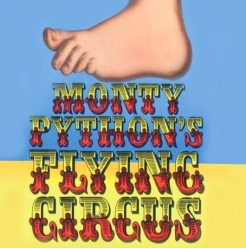
\includegraphics[width=0.5\textwidth]{./dados/figuras/mount-python.png}
    \fonte{\citeonline{MountPython}}
    \label{fig:figura-mountPython}
\end{figure}

\section{COMUNIDADE}

A primeira “comunidade” do Python surgiu formalmente com a criação do \textit{newsgroup: comp.lang.python na Usenet}, em março de 1993.
Posteriormente, este \textit{newsgroup} foi migrado para uma lista de discussão por e-mail, tendo como base o \textit{GNU Mailman}, um gerenciador de listas software livre escrito em Python.
\par No verão de 1994, o grupo iniciou uma discussão intitulada “Se Guido fosse atingido por um ônibus?”\footnote{
    \citeonline[p. ~1]{bus}
}.
Por mais mórbido que essa discussão soava, ela tocava no âmago da comunidade Python, pois Guido era seu principal desenvolvedor e ele tomava as decisões, criando assim o medo do Python desaparecer com seu criador.
Muitos justificavam que a política de “um homem só” reduziam as possibilidades de doação e investimento na linguagem.
Visto isso, nesta discussão, nasceu a necessidade de se criar um padrão ou organização responsável pelo Python, desvinculando Guido como o único responsável (e detentor de seus direitos) e garantindo assim a existência prolongada da linguagem.
 
No início de 2000, Guido, Barry Warsaw, Jeremy Hylton e Fred Drake receberam o convite para ser juntar à \textit{startup} BeOpen.com, uma iniciativa que estava recrutando diversos desenvolvedores \textit{Open Source}.
Antes de deixar a CNRI\footnote{
    A Corporation for National Research Initiatives (CNRI) é uma organização sem fins lucrativos formada em 1986 localizada em Virginia, Estados Unidos.
    Com o objetivo de empreender, fomentar e promover pesquisas de interesse público, as atividades giram em torno do desenvolvimento estratégico de tecnologias de informação baseadas em rede.
    A instituição fornece liderança e financiamento para pesquisa e desenvolvimento de infraestrutura de informação.\citeonline{cnri}
} os desenvolvedores foram forçados a lançar a versão 1.6, para finalizar o ciclo de desenvolvimento do Python.

Para a versão 1.6 a CNRI insistiu em utilizar uma licença escrita pelos seus próprios advogados.
Como esperado, esta licença diferia da utilizada até o momento, visando controlar “os direitos do Python” e submetendo o software às leis do estado da Virginia.
Como o Python era utilizado pelo GNU Mailman, a FSF (Free Software Foundation) estava receosa que essa nova licença pudesse restringir o uso de ambos os softwares. 
Desta forma, Richard Stallman e Eben Moglen (ambos da PSF\footnote{
    Vide: página \pageref{sec:python-software-foundation}, secção: \textit{Python Software Foundation}
}), analisaram a licença e chegaram a conclusão de que esta não era uma licença compatível com as premissas do software livre.
Com o apoio de Eric Raymond e da PSF a licença foi reescrita para satisfazer tanto a FSF quanto a CNRI.
A versão 1.6 foi lançada em Setembro de 2000, sendo que o grupo de desenvolvedores já estavam na BeOpen.com desde Maio de 2000.
\begin{figure}[!htb]
    \centering
    \caption{Free Software Foundation's Logo}
    
\includegraphics[width=0.5\textwidth]{./dados/figuras/FSF.png}
    \fonte{\citeonline{FSF}}
    \label{fig:figura-fsf}
\end{figure}

Devido a esta história do Python, a licença do Python era vista “em camadas”.
Na base tínhamos a licença do CWI, seguida pela licença do CNRI (no meio) e por último a licença da BeOpen.com.
Apesar da confusão, a licença era compatível com o modelo OSI que define uma licença Open Source e também é compatível com a GNU GPL (General Public License), garantindo as liberdades de um software livre.

\section{\textit{BeOpen.com} \& \textit{Digital Creations}}
Ja na BeOpen.com foi formado o grupo PythonLabs e a versão 2.0 do Python foi lançada em outubro de 2000.
O Python 2.0\footnote{
    A estadia na BeOpen.com rendeu apenas uma release do Python, a versão 2.0 citada anteriormente, pois em Outubro de 2000 ocorreu a falência e desmembramento da BeOpen.com e o PythonLabs foi contratado pela empresa Digital Creations.
} utilizava uma versão alterada da licença presente na versão 1.6 (alterando apenas o responsável para BeOpen.com).
Nesta estadia o Python (como comunidade e linguagem) evoluiu significativamente:
\begin{itemize}
    \item Os desenvolvedores passaram a se focar exclusivamente para o Python
    \item O desenvolvimento foi centralizado, utilizando um servidor CVS no SourceForge
    \item Por volta de 30 pessoas possuíam acesso de commit
    \item Banco de dados de patches e bugs também eram hospedados no SourceForge
    \item Criação das PEPs (Python Enhancement Proposal)
\end{itemize}

\begin{figure}[!htb]
    \centering
    \caption{Zope Logo}
    
\includegraphics[width=0.5\textwidth]{./dados/figuras/zope.png}
    \fonte{\citeonline{zope}}
    \label{fig:figura-zope}
\end{figure}

Em paralelo à esta contratação [\textit{Digital Creations}], o PythonLabs recebeu também convites de outras duas empresas, a VA Linux e a ActiveState.
Posteriormente a Digital Criations mudou de nome e ficou conhecida como Zope Corporation, referência ao seu produto mais conhecido, o Web CMS (Content Managing System) Zope.
Parte da mudança para da Zope Corporaton foi influenciada pela certeza de que o futuro do Python não podia ser influenciado pelos objetivos e ideais daqueles para os quais Guido trabalhava.
Foi então que criaram a Python Software Foundation (PSF).

\section{\textit{Python Software Foundation}}
\label{sec:python-software-foundation}
Python Software Foundation
Em 2001 foi criada a Python Software Foundation (PSF), uma organização sem fins lucrativos constituída por membros da equipe de desenvolvimento (daquela época) e por Eric Raymond.
Ela tem como objetivo ser dona de qualquer propriedade intelectual relacionada ao Python, e como missão promover e proteger o avanço da linguagem Python, além suportar e auxiliar o crescimento de comunidades de programadores Python.
Ela possui diversos patrocinadores como:
\begin{itemize}
    \item ActiveState;
    \item Advanced Simulation Technology Inc. (ASTi);
    \item Array BioPharma, Inc.;
    \item BizRate.com;
    \item Canonical;
    \item Globo;
    \item Google;
    \item Lucasfilm;
    \item Microsoft;
    \item OpenEye Scientific Software;
    \item O’Reilly Media, Inc.;
    \item Red Hat;


\end{itemize}
 
 
Em dezembro de 2008 é lançada a versão 3 do Python, mas ainda manteve muitos adeptos na versão 2, tanto que ambas são retrocompatíveis apesar da 2ª não ser mais recomendada para novos projetos.
 
 
Após a criação da PSF todas as \textit{releases} desde a 2.1 foram feitas utilizando a PSF License Agreement, uma licença que atribui todos os direitos do Python à PSF.
A licença está disponível na íntegra na documentação oficial do Python.
Uma vez que o futuro do Python (e a sua evolução) se desvinculou dos empregadores de seu criado, existem poucos relatos e registros.
Segue alguns destaques:
\begin{itemize} 
    \item Em Julho de 2003 o PythonLab saiu da Zope Corporation para trabalhar na Elemental Security em San Mateo, California;
    \item Em Dezembro de 2005 Guido foi trabalhar no Google em Mountain View, Califórnia;
    \item Em Janeiro de 2013 Guido foi trabalhar para o Dropbox.
\end{itemize}
         % Revisão de Literatura
% METODOLOGIA------------------------------------------------------------------

\chapter{PARADIGMA}
\label{chap:paradigma}

\section{CONSTRUÇÕES}
\label{sec:construcoes}

Construções de Python incluem: estrutura de seleção \textit{(if, else, elif)};
estrutura de repetição \textit{(for, while)}, que itera por um container, capturando cada elemento em uma variável local dada;
construção de classes (class); construção de sub-rotinas \textit{(def)};
construção de escopo \textit{(with)}, como por exemplo para adquirir um recurso.

\begin{figure}[!htb]
    \centering
    \caption{Python 3 The Standard type hyerarchy}
    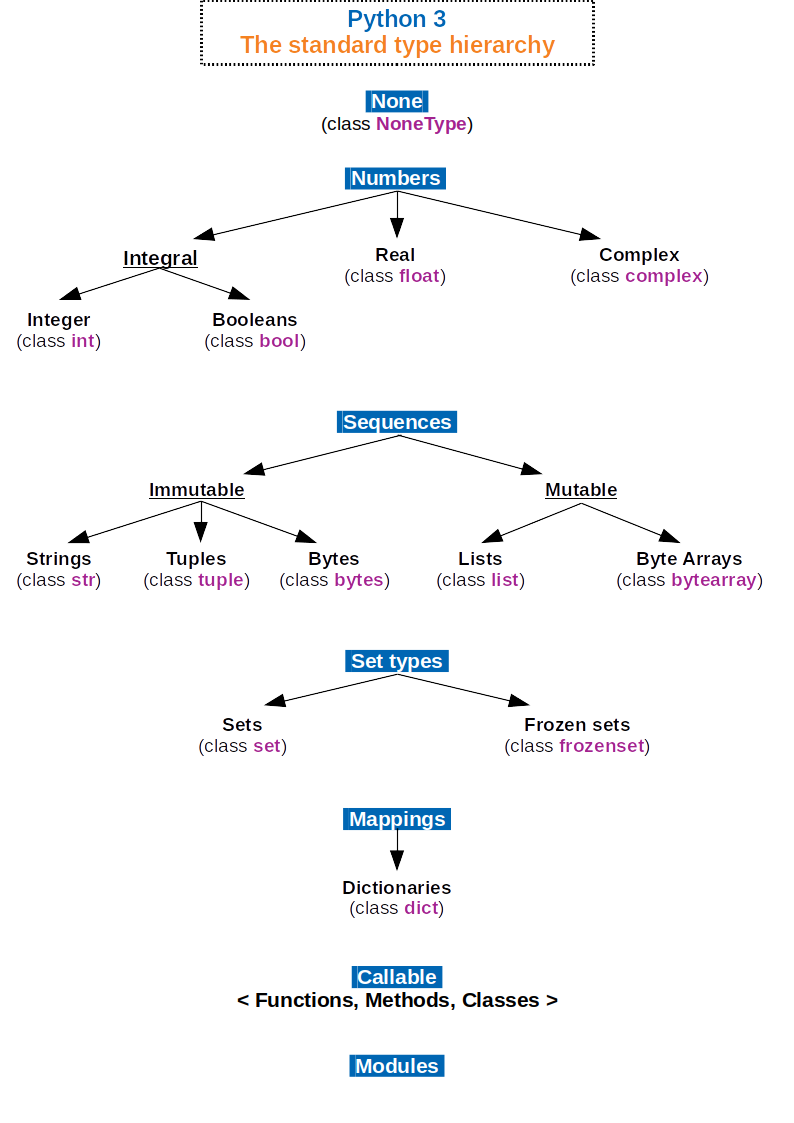
\includegraphics[width=0.75\textwidth]{./dados/figuras/Python_3._The_standard_type_hierarchy.png}
    \fonte{\url{https://pt.wikipedia.org/wiki/Ficheiro:Python_3._The_standard_type_hierarchy.png}}
    \label{fig:figura-tipos-python}
\end{figure}

\section{TIPOS DE DADOS}
\label{sec:tiposDados}

A tipagem de Python é forte, pois os valores e objetos têm tipos bem definidos e não sofrem coerções como em C ou Perl.
São disponibilizados diversos tipos de dados nativos:\footnote{
    O tipo int (inteiro) é transparentemente convertido para long caso não caiba em um int.
}
\footnote{
    Os Tipos set e frozenset não contém elementos duplicados
}

\begin{table}[!htb]
    \centering
    \caption[Tipos de dados em Python]{Tipos de dados em Python.
    \label{tab:tipos-dados}}
    \begin{tabular}{rrrrr}
        \toprule
        Tipo de dados & Descrição & Exemplo de sintaxe \\
        \midrule
        str, unicode    & Uma cadeia de caracteres imutável & 'foo'; "bar"  \\
        list    & Lista heterogênea mutável & [4.0, 'string', True]  \\
        tuple    & Tupla imutável & (4.0, 'string', True)  \\
        set, frozenset    & Conjunto não ordenado & set([4.0, 'string', True])  \\
        dict    & conjunto associativo & \{'key1': 1.0, 'key2': False\}  \\
        int    & Número de precisão fixa & 42; 2147483648L \\
        float    & Ponto flutuante & 3.1415927  \\
        complex    & Número complexo & $3+2j$  \\
        bool    & Booleano & True; False  \\
        $!=$    & Diferente & Diferente  \\
        \bottomrule
    \end{tabular}
    \fonte{\citeonline{PyDoc}}
\end{table}

Python também permite a definição dos tipos de dados próprios, através de classes.
Instâncias são construídas invocando a classe \textit{(FooClass())}, e as classes são instância da classe type, o que permite metaprogramação e reflexão.
Métodos são definidos como funções anexadas à classe, e a sintaxe \textit{instância.método(argumento)} é um atalho para \textit{Classe.método(instância, argumento)}.
Os métodos devem referenciar explicitamente a referência para o objeto incluindo o parâmetro self como o primeiro argumento do método.
Antes da versão 3.0, Python possuía dois tipos de classes: "old-style" e "new-style". Classes old-style foram eliminadas no Python 3.0, e todas são new-style. Em versões entre 2.2 e 3.0, ambos tipos de classes podiam ser usadas. A sintaxe de ambos estilos é a mesma, a diferença acaba sendo de onde objeto da classe é herdado, direta ou indiretamente (todas classes new-style herdam de objeto e são instâncias de type).
As classes new-styles nada mais são que tipos definidos pelo usuário.

\section{PALAVRAS RESERVADAS}
O Python 3 define as seguintes palavras reservadas:
\begin{itemize}
    \item \textbf{False}
    \item \textbf{None}
    \item \textbf{True}
    \item \textbf{and}
    \item \textbf{as}
    \item \textbf{assert}
    \item \textbf{break}
    \item \textbf{class}
    \item \textbf{continue}
    \item \textbf{def}
    \item \textbf{del}
    \item \textbf{elif}
    \item \textbf{else}
    \item \textbf{except}
    \item \textbf{finally}
    \item \textbf{for}
    \item \textbf{from}
    \item \textbf{global}
    \item \textbf{if}
    \item \textbf{import}
    \item \textbf{in}
    \item \textbf{is}
    \item \textbf{lambda}
    \item \textbf{not}
    \item \textbf{nonlocal}
    \item \textbf{or}
    \item \textbf{pass}
    \item \textbf{raise}
    \item \textbf{try}
    \item \textbf{return}
    \item \textbf{while}
    \item \textbf{with}
    \item \textbf{yield}
\end{itemize}

\section{OPERADORES}
Os operadores básicos de comparação como $==$, $<$, $>=$, entre outros são usados em todos os tipos de dados, como números, cadeias de texto, listas e mapeamentos.
Comparações em cadeia como $a < b < c$ possuem o mesmo significado básico que na matemática: os termos são comparadas na ordem.
É garantido que o processamento da expressão lógica irá terminar tão cedo o veredito seja claro, o princípio da avaliação mínima.
Usando a expressão anterior, se $a < b$ é falso, $c$ não é avaliado.
\par Quanto aos operadores lógicos, até Python 2.2 não havia o tipo de dado booleano.
Em todas as versões da linguagem os operadores lógicos\footnote{
    Na versão 2.2.1 as constantes True e False foram adicionadas (subclasses de 1 e 0 respectivamente)
} tratam \textit{"", 0, None, 0.0, [] e {}} como falso, enquanto o restante é tratado como verdadeiro de modo geral.
A comparação binária retorna uma das duas constantes acima.
\par Os operadores booleanos and e or também seguem a avaliação mínima. Por exemplo, $y == 0 or x/y > 100$ nunca lançará a exceção de divisão por zero.

\section{INTERPRETADOR INTERATIVO}
O interpretador interativo é uma característica diferencial da linguagem, porque há a possibilidade de testar o código de um programa e receber o resultado em tempo real, antes de iniciar a compilação ou incluí-las nos programas. 
Por exemplo:\footnote{
    A partir da versão 3.0, o comando print passou a ser uma função, sendo obrigatório o uso de parênteses.
}\\
\begin{algorithm}
    \caption{Exemplo do Interpretador Interativo}
    $>>>$ 1+1\\
    2\\
    $>>>$\\
    $>>>$ a = 1+1\\
    $>>>$ \textbf{print} a\\
    2\\
    $>>>$ \textbf{print}(a)\\
    2\\
    $>>>$\\
\end{algorithm}



                   % Metodologia
% RESULTADOS-------------------------------------------------------------------

\chapter{CARACTERÍSTICAS MARCANTES}
\section{ANÁLISE LÉXICA}
De acordo com \citeonline{10.5555/2011965}, a análise léxica é uma análise do interpretador, os programas são lidos por um analisador sintático que divide o código em \textit{tokens}.
Todo programa é dividido em linhas lógicas que são separadas pelo \textit{token NEWLINE}, as linhas físicas são trechos de código divididos pelo caractere \textit{ENTER}.
Linhas lógicas não podem ultrapassar linhas físicas com exceção de junção de linhas, por exemplo:

\begin{algorithm}
    \caption{Exemplo do Interpretador Interativo}
    \textbf{if} resultado > 2 \textbf{and} 1 <= 5  \textbf{and} 2 < 5:\\
    \textbf{print}('Resultado: \%f' \% d)\\
ou\\
MESES COMO $= ['janeiro', 'fevereiro', 'março',$\\
                $'abril',   'maio',      'junho',$\\
               $ 'julho',   'agosto',    'setembro',$\\
                $'outubro', 'novembro',  'dezembro']$\\
\end{algorithm}


Para a delimitação de blocos de códigos, os delimitadores são colocados em uma pilha e diferenciados por sua indentação, iniciando a pilha com valor 0 (zero) e colocando valores maiores que os anteriores.
Para cada começo de linha, o nível de indentação é comparado com o valor do topo da pilha.
\begin{itemize}
    \item Se o número da linha for igual ao topo da pilha, a pilha não é alterada.
    \item Se o valor for maior, a pilha recebe o nível de indentação da linha e o nome \textit{INDENT (psuh)}.
    \item Se o nível de indentação for menor, então é desempilhado até chegar a um nível de indentação recebendo o nome \textit{DEDENT (pop)}.
    \item Se não encontrar nenhum valor, é gerado um erro de indentação.
\end{itemize}
\par Abaixo um exemplo de permutação, retirado do capítulo 2.1 sobre Estrutura de linhas na Análise léxica do Manual de Referência da linguagem\footnote{
    \citeonline[p. ~37]{10.5555/2011965}, vide figura \ref{fig:figura-ident-python}: p. \pageref{fig:figura-ident-python}, seção: ANÁLISE LÉXICA
}:

\begin{figure}[!htb]
    \centering
    \caption{Indentação em Python}
    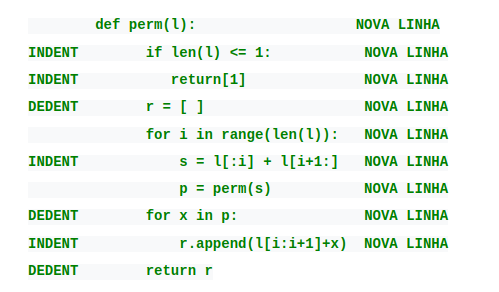
\includegraphics[width=0.75\textwidth]{./dados/figuras/ident1.png}
    \fonte{\citeonline{10.5555/2011965}}
    \label{fig:figura-ident-python}
\end{figure}

Python foi desenvolvido para ser uma linguagem de fácil leitura, com um visual agradável, frequentemente usando palavras e não pontuações como em outras linguagens.
Para a separação de blocos de código, a linguagem usa espaços em branco e indentação ao invés de delimitadores visuais como chaves (C, Java) ou palavras (BASIC, Fortran, Pascal).
Diferente de linguagens com delimitadores visuais de blocos, em Python a indentação é obrigatória.
O aumento da indentação indica o início de um novo bloco, que termina da diminuição da indentação.
\par Usando um editor de texto comum é muito fácil existirem erros de indentação, o recomendado é configurar o editor conforme a análise léxica do Python ou utilizar uma IDE.
Todas as IDE que suportam a linguagem fazem indentação automaticamente.\\    
Exemplo:

\begin{figure}[!htb]
    \centering
    \caption{Indentação em Python}
    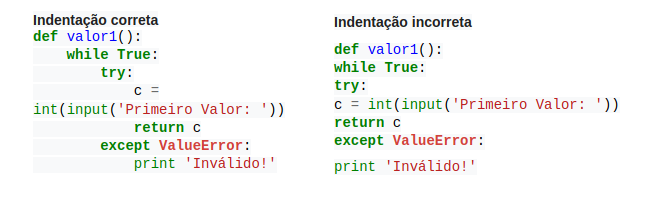
\includegraphics[width=0.75\textwidth]{./dados/figuras/ident2.png}
    \fonte{\citeonline{10.5555/2011965}}
    \label{fig:figura-ident2-python}
\end{figure}

O analisador léxico reconhecerá as palavras reservadas while, def, try, except, return, print e as cadeias de caracteres entre aspas simples e a indentação, e se não houver problemas o programa executará normalmente, senão apresentará a exceção: \textit{IndentationError\footnote{
    \citeonline[p. ~20]{pyMan}
}}.

\section{COMPILADOR DE BYTECODE}
A linguagem é de altíssimo nível, como já dito, mas ela também pode compilar seus programas para que a próxima vez que o executar não precise compilar o novamente, reduzindo o tempo de carga na execução.
\par Utilizando o interpretador interativo não é necessário a criação do arquivo de Python compilado, os comandos são executados interativamente.
Entretanto, quando um programa ou um módulo é evocado, o interpretador realiza a análise léxica e sintática, compila o código de alto nível se necessário e o executa na máquina virtual da linguagem.
\par O bytecode é armazenado em arquivos com extensão \textit{.pyc ou .pyo}, este último no caso de bytecode otimizado\footnote{
    Interessante notar que o bytecode da linguagem também é de alto nível, ou seja, é mais legível aos seres humanos que o código de byte do C, por exemplo.}.
\par Normalmente, o Python trabalha com dois grupos de arquivos:

\begin{itemize}
    \item Os módulos do núcleo da linguagem, sua biblioteca padrão e os módulos independentes, criados pelo usuário.
    \item No núcleo do interpretador existe o analisador léxico, o analisador sintático que utiliza Estruturas de Objetos (tempo de execução), o Compilador que aloca memória (tempo de execução) e depois do Avaliador de código que modifica o estado atual do programa (tempo de execução), mostrando resultado para o usuário.
\end{itemize}

\section{ORIENTAÇÃO A OBJETO}
Python suporta a maioria das técnicas da programação orientada a objeto.
Qualquer objeto pode ser usado para qualquer tipo, e o código funcionará enquanto haja métodos e atributos adequados.
O conceito de objeto na linguagem é bastante abrangente: classes, funções, números e módulos são todos considerados objetos.
Também há suporte para metaclasses, polimorfismo, e herança (inclusive herança múltipla).
Há um suporte limitado para variáveis privadas.

\par Na versão 2.2 de Python foi introduzido um novo estilo de classes em que objetos e tipos foram unificados, permitindo a especialização de tipos.
Já a partir da versão 2.3 foi introduzido um novo método de resolução de ambiguidades para heranças múltiplas.\cite{30}

Uma classe é definida com \textit{class} nome, e o código seguinte é a composição dos atributos.
Todos os métodos da classe recebem uma referência a uma instância da própria classe como seu primeiro argumento, e a convenção é que se chame este argumento self.
Assim os métodos são chamados objeto.método(argumento1, argumento2) e são definidos iguais a uma função, como método(self, argumento1, argumento2).
Veja que o parâmetro self conterá uma referência para a instância da classe definida em objeto quando for efetuada esta chamada.
Os atributos da classe podem ser acessados em qualquer lugar da classe, e os atributos de instância (ou variável de instância) devem ser declarados dentro dos métodos utilizando a referência à instância atual (self)

Em Python não existe proteção dos membros duma classe ou instância pelo interpretador, o chamado encapsulamento.
Convenciona-se que atributos com o nome começando com um são de uso privado da classe, mas não há um policiamento do interpretador contra acesso a estes atributos.
Uma exceção são nomes começando com, no caso em que o interpretador modifica o nome do atributo.

\par Python permite polimorfismo, que condiz com a reutilização de código.
É fato que funções semelhantes em várias partes do software sejam utilizadas várias vezes, então definimos esta função como uma biblioteca e todas as outras funções que precisarem desta a chamam sem a necessidade de reescrevê-la.

\par Python não possui overloading; não é possível criar duas funções com o mesmo nome, pois elas são consideradas atributos da classe.
Caso o nome da função se repita em outra assinatura, o interpretador considera esta última como override e sobrescreve a função anterior.
Algumas operações entre diferentes tipos são realizadas através de coerção ($ex.: 3.2 + 3$).

\par É possível encapsular abstrações em módulos e pacotes. Quando um arquivo é criado com a extensão \textit{.py}, ele automaticamente define um módulo.
Um diretório com vários módulos é chamado de pacote e deve conter um modulo chamado $\_\_init\_\_$, para defini-lo como principal.
Estas diferenciações ocorrem apenas no sistema de arquivos. Os objetos criados são sempre módulos.
Caso o código não defina qual dos módulos será importado, o padrão é o $\_\_init\_\_$.

\section{PROGRAMAÇÃO FUNCIONAL}
Uma das construções funcionais de Python é a compreensão de listas\footnote{
    Compreensão de lista é uma construção sintática disponível em algumas linguagens de programação para criação de uma lista baseada em listas existentes.
    Ela segue a forma da notação de definição de conjunto matemática (compreensão de conjunto) como forma distinta para uso de funções de mapa e filtro. \citeonline{list}
}, uma forma eficiente de construir listas.
Por exemplo, pode-se usar a técnica para calcular as cinco primeiras potências de dois.
O algoritmo quicksort também pode ser expresso usando a mesma técnica.

Em Python, funções são objetos de primeira classe que podem ser criados e armazenados dinamicamente.
O suporte a funções anônimas está na construção lambda (Cálculo-$\lambda$).
Não há disponibilidade de funções anônimas de fato, pois os lambdas contêm somente expressões e não blocos de código.

Python também suporta clausuras léxicas desde a versão 2.2.
Já geradores foram introduzidos na versão 2.2 e finalizados na versão 2.3, e representam o mecanismo de Python para a avaliação preguiçosa\footnote{
    Avaliação preguiçosa (também conhecida por avaliação atrasada) é uma técnica usada em programação para atrasar a computação até um ponto em que o resultado da computação é considerado suficiente, o necessário.
Os benefícios da avaliação preguiçosa incluem o aumento do desempenho ao evitar cálculos desnecessários, evitando condições de erro na avaliação de expressões compostas, a habilidade em construir estruturas de dados infinitas e a habilidade de definir estruturas do controle como funções regulares melhor que usando primitivas internas.
No oposto de avaliação atrasada está avaliação ansiosa, também conhecido como avaliação rigorosa. \citeonline{pldc}
} de funções. 


\section{TRATAMENTO DE EXCEÇÕES}

Python suporta e faz uso constante de tratamento de exceções como uma forma de testar condições de erro e outros eventos inesperados no programa.
É inclusive possível capturar uma exceção causada por um erro de sintaxe.
O estilo da linguagem apoia o uso de exceções sempre que uma condição de erro pode aparecer.
Por exemplo, ao invés de testar a disponibilidade de acesso a um recurso, a convenção é simplesmente tentar usar o recurso e capturar a exceção caso o acesso seja rejeitado.

\par Exceções são usadas frequentemente como uma estrutura de seleção, substituindo blocos \textit{if-else}, especialmente em situações que envolvem threads.
Uma convenção de codificação é o EAFP, do inglês, “é mais fácil pedir perdão que permissão”.
Isso significa que, em relação a desempenho, é preferível capturar exceções do que testar atributos antes de os usar.
Segue abaixo exemplos de código que testam atributos e que capturam exceções:

\begin{figure}[!htb]
    \centering
    \caption{Mount Python’s Logo}
    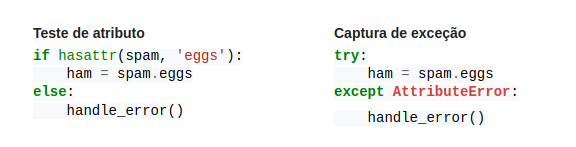
\includegraphics[width=1\textwidth]{./dados/figuras/tryCatch.png}
    \fonte{\citeonline{10.5555/2011965}}
    \label{fig:figura-mountPython}
\end{figure}

\par Ambos os códigos produzem o mesmo efeito, mas há diferenças de desempenho.
Quando spam possui o atributo eggs, o código que captura exceções é mais rápido.
Caso contrário, a captura da exceção representa uma perda considerável de desempenho, e o código que testa o atributo é mais rápido.
Geralmente, o paradigma da captura de exceções é mais rápido, e também pode evitar problemas de concorrência.
Por exemplo, num ambiente multitarefa, o espaço de tempo entre o teste do atributo e seu uso de fato pode invalidar o atributo, problema que não acontece no caso da captura de exceções.

\section{BIBLIOTECA PADRÃO}
Python possui uma grande biblioteca padrão\footnote{
    Algumas partes da biblioteca são cobertas por especificações (por exemplo, a implementação WSGI da wsgiref segue o PEP 333), mas a maioria dos módulos não o segue.
}, geralmente citada como um dos maiores trunfos da linguagem, fornecendo ferramentas para diversas tarefas.
Por conta da grande variedade de ferramentas fornecida pela biblioteca padrão, combinada com a habilidade de usar linguagens de nível mais baixo como C e C++, Python pode ser poderosa para conectar componentes diversos de software.

A biblioteca padrão conta com facilidades para escrever aplicações para a Internet, contando com diversos formatos e protocolos como MIME e HTTP.
Também há módulos para criar interfaces gráficas, conectar em bancos de dados relacionais e manipular expressões regulares.

\section{INTEROPERABILIDADE}
Outro ponto forte da linguagem é sua capacidade de interoperar com várias outras linguagens, principalmente código nativo.
A documentação da linguagem inclui exemplos de como usar a Python C-API para escrever funções em C\footnote{
    Mas atualmente esse \textit{sequer} é o modo mais indicado de interoperação, havendo alternativas tais como Cython, Swig ou cffi
} que podem ser chamadas diretamente de código Python.
A biblioteca Boost do C++ inclui uma biblioteca para permitir a interoperabilidade entre às duas linguagens, e pacotes científicos usam bibliotecas de alto desempenho numérico escritos em Fortran e mantidos há décadas.

\section{COMENTÁRIOS}
Python fornece duas alternativas para documentar o código.
A primeira é o uso de comentários para indicar o que certo código faz.
Comentários começam com \# e são terminados pela quebra da linha.
Não há suporte para comentários que se estendem por mais de uma linha; cada linha consecutiva de comentário deve indicar \#.
A segunda alternativa é o uso de cadeias de caractere, literais de texto inseridos no código sem atribuição.
Cadeias de caracteres em Python são delimitadas por $"$ ou $'$ para única linha e por $"""$ ou $'''$ para múltiplas linhas.
Entretanto, é convenção usar os métodos de múltiplas linhas em ambos os casos.

Diferente de comentários, as cadeias de caracteres usadas como documentação são objetos Python e fazem parte do código interpretado.
Isso significa que um programa pode acessar sua própria documentação e manipular a informação.
Há ferramentas que extraem automaticamente essa documentação para a geração da documentação de API a partir do código.
Documentação através de cadeias de caracteres também pode ser acessada a partir do interpretador através da função \textit{help()}.                    % Resultados
\chapter{LINGUAGENS SIMILARES OU CONFLITANTES}


Python é frequentemente comparado a outras linguagens interpretadas, como Java, JavaScript, Perl, Tcl, Smalltalk, C++, Common Lisp e Scheme\cite{comparacao}.
Na prática, a escolha de uma linguagem de programação é frequentemente ditada por outras restrições reais, como custo, disponibilidade, treinamento e investimento inicial e até mesmo compromisso emocional.

O subconjunto “baseado em objeto” do Python é equivalente ao JavaScript e, como o JS, o Python suporta um estilo de programação que usa funções e variáveis simples sem se envolver em definições de classe.
No entanto, para JavaScript, isso é tudo o que existe.

Espera-se que os programas Python sejam mais lentos do que os programas Java, porém levam menos tempo para serem desenvolvidos.
Os programas Python são tipicamente 3 a 5 vezes mais baixos do que programas Java comparáveis.
Essa diferença pode ser atribuída aos tipos de dados de alto nível integrados do Python e sua tipagem dinâmica.
Devido à digitação em tempo de execução, o tempo de execução do Python terá um desempenho melhor do que o Java.
Por exemplo, ao avaliar a expressão a + b, você deve primeiro examinar os objetos AEB para descobrir seu tipo, que é desconhecido em tempo de compilação.
Por essas razões, Python é muito mais adequado como uma linguagem "cola", enquanto Java é melhor caracterizado como uma linguagem de implementação de baixo nível.
Na verdade, os dois juntos formam uma ótima combinação.
Os componentes podem ser desenvolvidos em Java e combinados para formar aplicativos Python; Python também pode ser usado para prototipar componentes até que seu design possa ser "reforçado" em uma implementação Java.

Python brilha como uma linguagem de cola, usada para combinar componentes escritos em C++.
Como comparado em java, um programa tem de 3 a 5 vezes maior [nível], vemos essa diferença aumentar em relação de 5 a 10 vezes numa aplicação de C++ compara Python.

Por sua vez, o Tcl, que tradicionalmente armazena todos os dados como strings, é fraco em estruturas de dados e o código regular é executado muito mais devagar do que o Python.
Portanto, enquanto um grande aplicativo Tcl "típico" geralmente contém extensões Tcl escritas em C ou C ++ que são específicas para esse aplicativo, aplicativos Python equivalentes podem ser escritos em "Python puro".
Obviamente, o desenvolvimento puro em Python é muito mais rápido do que escrever e depurar um componente C ou C ++.
Python adotou a interface Tk como sua biblioteca padrão de componentes GUI.

Em Smalltalk, talvez a maior diferença entre eles seja a sintaxe "convencional" do Python, que oferece uma vantagem no treinamento de programadores.
No entanto, ele distingue os tipos de objeto embutidos das classes definidas pelo usuário e atualmente não permite a herança de tipos embutidos.
Python tem uma filosofia diferente em relação ao ambiente de desenvolvimento e distribuição de código. Enquanto Smalltalk tradicionalmente tem uma "imagem de sistema" monolítica, que inclui o ambiente e o programa do usuário, o Python armazena módulos padrão e módulos do usuário em arquivos individuais que podem ser facilmente reorganizados ou distribuídos fora do sistema.

Python e Perl vêm de um plano de fundo semelhante e possuem muitas características semelhantes, mas têm uma filosofia diferente.
Python enfatiza o suporte para metodologias de programação comuns, como desenho de estrutura de dados e programação orientada a objetos, e encoraja os programadores a escrever um código legível , fornecendo uma notação elegante, mas não excessivamente encriptada.

Em relação a common e lisp e Scheme, essas linguagens eram tão próximas dele em sua semântica dinâmica, mas tão diferentes em suas abordagens sintáticas que a comparação se tornou quase um argumento religioso: a falta de sintaxe de Lisp é vantagem ou desvantagem?
Deve-se notar que o Python possui recursos de introspecção semelhantes aos do Lisp e que os programas Python podem construir e executar fragmentos de programa em tempo real. Freqüentemente, as propriedades do mundo real são decisivas:
Common Lisp é grande e o mundo Scheme é fragmentado entre muitas versões incompatíveis, da qual Python tem uma implementação única, gratuita e compacta.

 
                   % Capítulo com Orientações de uso do Template
% % ORIENTAÇÕES GERAIS------------------------------------------------------------


% SOBRE AS ILUSTRAÇÕES----------------------------------------------------------
\chapter{SOBRE AS ILUSTRAÇÕES}
\label{chap:apSobreIlust}

A seguir exemplifica-se como inserir ilustrações no corpo do trabalho. As ilustrações serão indexadas automaticamente em suas respectivas listas. A numeração sequencial de figuras, tabelas e equações também ocorre de modo automático.

Referências cruzadas são obtidas através dos comandos \verb|\label{}| e \verb|\ref{}|. Sendo assim, não é necessário por exemplo, saber que o número de certo capítulo é \ref{chap:fundamentacaoTeorica} para colocar o seu número no texto. Outra forma que pode ser utilizada é esta: \autoref{chap:fundamentacaoTeorica}, facilitando a inserção, remoção e manejo de elementos numerados no texto sem a necessidade de renumerar todos esses elementos.

% FIGURAS-----------------------------------------------------------------------
\chapter{FIGURAS}
\label{chap:figuras}

Exemplo de como inserir uma figura. A \autoref{fig:figura-exemplo1} aparece automaticamente na lista de figuras. Para saber mais sobre o uso de imagens no \LaTeX{} consulte literatura especializada \cite{Goossens2007}.

Os arquivos das figuras devem ser armazenados no diretório de "/dados".

\begin{figure}[!htb]
    \centering
    \caption{Exemplo de Figura}
    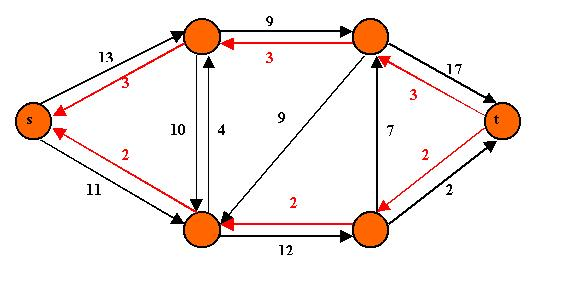
\includegraphics[width=0.5\textwidth]{./dados/figuras/figura1}
    \fonte{\citeonline{IRL2014}}
    \label{fig:figura-exemplo1}
\end{figure}

% QUADROS E TABELAS---------------------------------------------------------------
\chapter{QUADROS E TABELAS}
\label{chap:tabelas}

Exemplo de como inserir o \autoref{qua:quadro-exemplo1} e a \autoref{tab:tabela-exemplo1}. Ambos aparecem automaticamente nas suas respectivas listas. Para saber mais informações sobre a construção de tabelas no \LaTeX{} consulte literatura especializada \cite{Mittelbach2004}.

Ambos os elementos (Quadros e Tabelas) devem ser criados em arquivos separados para facilitar manutenção e armazenados no diretório de "/dados".

\begin{quadro}[!htb]
    \centering
    \caption{Exemplo de Quadro.\label{qua:quadro-exemplo1}}
    \begin{tabular}{|p{7cm}|p{7cm}|}
        \hline
        \textbf{BD Relacionais} & \textbf{BD Orientados a Objetos} \\
        \hline
        Os dados são passivos, ou seja, certas operações limitadas podem ser automaticamente acionadas quando os dados são usados. Os dados são ativos, ou seja, as solicitações fazem com que os objetos executem seus métodos. & Os processos que usam dados mudam constantemente. \\
        \hline
    \end{tabular}
    \fonte{\citeonline{Barbosa2004}}
\end{quadro}


A diferença entre quadro e tabela está no fato que um quadro é formado por linhas horizontais e verticais. Deve ser utilizado quando o conteúdo é majoritariamente não-numérico. O número do quadro e o título vem acima do quadro, e a fonte, deve vir abaixo. E Uma tabela é formada apenas por linhas verticais. Deve ser utilizada quando o conteúdo é majoritariamente numérico. O número da tabela e o título vem acima da tabela, e a fonte, deve vir abaixo, tal como no quadro.

\begin{table}[!htb]
    \centering
    \caption[Resultado dos testes]{Resultado dos testes.
    \label{tab:tabela-exemplo1}}
    \begin{tabular}{rrrrr}
        \toprule
            & Valores 1 & Valores 2 & Valores 3 & Valores 4 \\
        \midrule
            Caso 1 & 0,86 & 0,77 & 0,81 & 163 \\
            Caso 2 & 0,19 & 0,74 & 0,25 & 180 \\
            Caso 3 & 1,00 & 1,00 & 1,00 & 170 \\
        \bottomrule
    \end{tabular}
    \fonte{\citeonline{Barbosa2004}}
\end{table}


% EQUAÇÕES-----------------------------------------------------------------------
\chapter{EQUAÇÕES}
\label{chap:equacoes}

Exemplo de como inserir a \autoref{eq:equacao-exemplo1} e a Eq. \ref{eq:equacao-exemplo2} no corpo do texto \footnote{Deve-se atentar ao fato de a formatação das equações ficar muito boa esteticamente.}. Observe que foram utilizadas duas formas distintas para referenciar as equações.

\begin{equation}
    X(s) = \int\limits_{t = -\infty}^{\infty} x(t) \, \text{e}^{-st} \, dt
    \label{eq:equacao-exemplo1}
\end{equation}

\begin{equation}
    F(u, v) = \sum_{m = 0}^{M - 1} \sum_{n = 0}^{N - 1} f(m, n) \exp \left[ -j 2 \pi \left( \frac{u m}{M} + \frac{v n}{N} \right) \right]
    \label{eq:equacao-exemplo2}
\end{equation}

% ALGORITMOS-----------------------------------------------------------------------
\chapter{ALGORITMOS}
\label{chap:algoritmos}

Exemplo de como inserir um algoritmo. Para inserção de algoritmos utiliza-se o pacote {\ttfamily algorithm2e} que já está devidamente configurado dentro do template.

Os algoritmos devem ser criados em arquivos separados para facilitar manutenção e armazenados no diretório de "/dados".\\
\\

\begin{algorithm}
    \caption{Exemplo de Algoritmo}
    \KwIn{o número $n$ de vértices a remover, grafo original $G(V, E)$}
    \KwOut{grafo reduzido $G'(V,E)$}
    $removidos \leftarrow 0$ \\
    \While {removidos $<$ n } {
        $v \leftarrow$ Random$(1, ..., k) \in V$ \\
            \For {$u \in adjacentes(v)$} {
                remove aresta (u, v)\\
                $removidos \leftarrow removidos + 1$\\
            }
            \If {há  componentes desconectados} {
                remove os componentes desconectados\\
            }
        }
\end{algorithm}


% SOBRE AS LISTAS--------------------------------------------------------------------
\chapter{SOBRE AS LISTAS}
\label{chap:apSobreLista}

Para construir listas de "\textit{bullets}"{} ou listas enumeradas, inclusive listas aninhadas, é utilizado o pacote \verb|paralist|.

Exemplo de duas listas não numeradas aninhadas, utilizando o comando \verb|\itemize|. Observe a indentação, bem como a mudança automática do tipo de "\textit{bullet}"{} nas listas aninhadas.

\begin{itemize}
    \item item não numerado 1
    \item item não numerado 2
    \begin{itemize}
        \item subitem não numerado 1
        \item subitem não numerado 2
        \item subitem não numerado 3
    \end{itemize}
    \item item não numerado 3
\end{itemize}

Exemplo de duas listas numeradas aninhadas, utilizando o comando \verb|\enumerate|. Observe a numeração progressiva e indentação das listas aninhadas.

\begin{enumerate}
    \item item numerado 1
    \item item numerado 2
    \begin{enumerate}
        \item subitem numerado 1
        \item subitem numerado 2
        \item subitem numerado 3
    \end{enumerate}
    \item item numerado 3
\end{enumerate}

% SOBRE AS CITAÇÕES E CHAMADAS DE REFERÊNCAS----------------------------------------------
\chapter{SOBRE AS CITAÇÕES E CHAMADAS DE REFERÊNCAS}
\label{chap:apSobreCita}

Citações são trechos de texto ou informações obtidas de materiais consultadss quando da elaboração do trabalho. São utilizadas no texto com o propósito de esclarecer, completar e embasar as ideias do autor. Todas as publicações consultadas e utilizadas (por meio de citações) devem ser listadas, obrigatoriamente, nas referências bibliográficas, para preservar os direitos autorais. São classificadas em citações indiretas e diretas.

% CITAÇÕES INDIRETAS-----------------------------------------------------------------------
\chapter{CITAÇÕES INDIRETAS}
\label{chap:citacoesLivres}

É a transcrição, com suas próprias palavras, das idéias de um autor, mantendo-se o sentido original. A citação indireta é a maneira que o pesquisador tem de ler, compreender e gerar conhecimento a partir do conhecimento de outros autores. Quanto à chamada da referência, ela pode ser feita de duas maneiras distintas, conforme o nome do(s) autor(es) façam parte do seu texto ou não. Exemplo de chamada fazendo parte do texto:\\
\\Enquanto \citeonline{Maturana2003} defendem uma epistemologia baseada na biologia. Para os autores, é necessário rever \ldots.\\

A chamada de referência foi feita com o comando \verb|\citeonline{chave}|, que produzirá a formatação correta.

A segunda forma de fazer uma chamada de referência deve ser utilizada quando se quer evitar uma interrupção na sequência do texto, o que poderia, eventualmente, prejudicar a leitura. Assim, a citação é feita e imediatamente após a obra referenciada deve ser colocada entre parênteses. Porém, neste caso específico, o nome do autor deve vir em caixa alta, seguido do ano da publicação. Exemplo de chamada não fazendo parte do texto:\\
\\Há defensores da epistemologia baseada na biologia que argumentam em favor da necessidade de \ldots \cite{Maturana2003}.\\

Nesse caso a chamada de referência deve ser feita com o comando \verb|\cite{chave}|, que produzirá a formatação correta.

% CITAÇÕES DIRETAS-----------------------------------------------------------------------
\chapter{CITAÇÕES DIRETAS}
\label{chap:citacoesLiterais}

É a transcrição ou cópia de um parágrafo, de uma frase, de parte dela ou de uma expressão, usando exatamente as mesmas palavras adotadas pelo autor do trabalho consultado.

Quanto à chamada da referência, ela pode ser feita de qualquer das duas maneiras já mencionadas nas citações indiretas, conforme o nome do(s) autor(es) façam parte do texto ou não. Há duas maneiras distintas de se fazer uma citação direta, conforme o trecho citado seja longo ou curto.

Quando o trecho citado é longo (4 ou mais linhas) deve-se usar um parágrafo específico para a citação, na forma de um texto recuado (4 cm da margem esquerda), com tamanho de letra menor e espaçamento entrelinhas simples. Exemplo de citação longa:
\\\begin{citacao}
    Desse modo, opera-se uma ruptura decisiva entre a reflexividade filosófica, isto é a possibilidade do sujeito de pensar e de refletir, e a objetividade científica. Encontramo-nos num ponto em que o conhecimento científico está sem consciência. Sem consciência moral, sem consciência reflexiva e também subjetiva. Cada vez mais o desenvolvimento extraordinário do conhecimento científico vai tornar menos praticável a própria possibilidade de reflexão do sujeito sobre a sua pesquisa \cite[p.~28]{Silva2000}.
\end{citacao}

Para fazer a citação longa deve-se utilizar os seguintes comandos:
\begin{verbatim}
\begin{citacao}
<texto da citacao>
\end{citacao}
\end{verbatim}

No exemplo acima, para a chamada da referência o comando \verb|\cite[p.~28]{Silva2000}| foi utilizado, visto que os nomes dos autores não são parte do trecho citado. É necessário também indicar o número da página da obra citada que contém o trecho citado.

Quando o trecho citado é curto (3 ou menos linhas) ele deve inserido diretamente no texto entre aspas. Exemplos de citação curta:\\
\\A epistemologia baseada na biologia parte do princípio de que "assumo que não posso fazer referência a entidades independentes de mim para construir meu explicar" \cite[p.~35]{Maturana2003}.\\
\\A epistemologia baseada na biologia de \citeonline[p.~35]{Maturana2003} parte do princípio de que "assumo que não posso fazer referência a entidades independentes de mim para construir meu explicar".

% DETALHES SOBRE AS CHAMADAS DE REFERÊNCIAS---------------------------------------------------------
\chapter{DETALHES SOBRE AS CHAMADAS DE REFERÊNCIAS}
\label{chap:referUtilizadas}

Outros exemplos de comandos para as chamadas de referências e o resultado produzido por estes:\\
\\\citeonline{Maturana2003} \ \ \  \verb|\citeonline{Maturana2003}|\\
\citeonline{Barbosa2004} \ \ \   \verb|\citeonline{Barbosa2004}|\\
\cite[p.~28]{Silva2000} \ \ \  \verb|\cite[p.~28]{Silva2000}|\\
\citeonline[p.~33]{Silva2000} \ \ \   \verb|\citeonline[p.~33]{v}|\\
\cite[p.~35]{Maturana2003} \ \ \   \verb|\cite[p.~35]{Maturana2003}|\\
\citeonline[p.~35]{Maturana2003} \ \ \   \verb|\citeonline[p.~35]{Maturana2003}|\\
\cite{Barbosa2004,Maturana2003} \ \ \   \verb|\cite{Barbosa2004,Maturana2003}|\\

% SOBRE AS REFERÊNCIAS BIBLIOGRÁFICAS-------------------------------------------------------
\chapter{SOBRE AS REFERÊNCIAS BIBLIOGRÁFICAS}
\label{chap:apSobreRefer}

A bibliografia é feita no padrão \textsc{Bib}\TeX{}. As referências são colocadas em um arquivo separado. Neste template as referências são armazenadas no arquivo "base-referencias.bib".

Existem diversas categorias documentos e materiais componentes da bibliografia. A classe abn\TeX{} define as seguintes categorias (entradas):

\begin{verbatim}
@book
@inbook
@article
@phdthesis
@mastersthesis
@monography
@techreport
@manual
@proceedings
@inproceedings
@journalpart
@booklet
@patent
@unpublished
@misc
\end{verbatim}

Cada categoria (entrada) é formatada pelo pacote \citeonline{abnTeX22014d} de uma forma específica. Algumas entradas foram introduzidas especificamente para atender à norma \citeonline{NBR6023:2002}, são elas: \verb|@monography|, \verb|@journalpart|,\verb|@patent|. As demais entradas são padrão \textsc{Bib}\TeX{}. Para maiores detalhes, refira-se a \citeonline{abnTeX22014d}, \citeonline{abnTeX22014b}, \citeonline{abnTeX22014c}.

% NOTAS DE RODAPÉ--------------------------------------------------------------------------
\chapter{NOTAS DE RODAPÉ}
\label{chap:notasRodape}

As notas de rodapé pode ser classificadas em duas categorias: notas explicativas\footnote{é o tipo mais comum de notas que destacam, explicam e/ou complementam o que foi dito no corpo do texto, como esta nota de rodapé, por exemplo.} e notas de referências. A notas de referências, como o próprio nome ja indica, são utilizadas para colocar referências e/ou chamadas de referências sob certas condições.
                   % Capítulo com Orientações de uso do Template
% CONCLUSÃO--------------------------------------------------------------------

\chapter{CONCLUSÃO}
\label{chap:conclusao}
\section{CONSIDERAÇÕES FINAIS}
\label{sec:consideracoesFinais}

Python é uma linguagem fascinante.
De acordo com o site Stack Overflow\footnote{
    O Stack Overflow survey é a maior pesquisa sobre programadores do mundo, no ano de 2020.
    "Este ano [2020], em vez de almejar ser o maior, nos propusemos a tornar nossa pesquisa mais representativa da diversidade de programadores em todo o mundo. 
    Dito isso, a pesquisa ainda é grande.
    A pesquisa deste ano foi realizada por quase 65.000 pessoas." \citeonline{SO}.
    Outra pesquisa relevante que também aponta resultados similares é a Interactive: The Top Programming Languages da IEEE, onde Python também é a mais usada \citeonline{SOIEEE}.
}, python é a linguagem mais amada e mais utilizada atualmente.
Com vários adeptos e uma rica comunidade, a linguagem continua em seu crescimento.
Ela é versátil em fazer programas rápidos, \textit{Data Science}, segurança da informação e diversas outras áreas, se tornando um “canivete suíço” da programação.
Apesar da sua popularidade recente (a partir do Python 2), ela era extensivamente utilizada em uma série de aplicações desde a década de 90.

Atualmente, Python começou a ser utilizado como linguagem introdutória por várias instituições de ensino sendo atualmente a mais recomendada para iniciantes, apesar do conhecimento de baixo nível não seja profundo.
Certamente, a linguagem possui um futuro promissor pela frente na inovação da área científica, educacional, entre outras.
                 			   % Conclusão

\postextual
% INSERE ELEMENTOS PÓS-TEXTUAIS
% REFERÊNCIAS------------------------------------------------------------------

% Carrega o arquivo "base-referencias.bib" e extrai automaticamente as referências citadas

\bibliography{./base-referencias}
\bibliographystyle{abntex2-alf} % Define o estilo ABNT para formatar a lista de referências
% OBSERVAÇÕES------------------------------------------------------------------
% Este arquivo não precisa ser alterado.
           			   % Referências
% APÊNDICES--------------------------------------------------------------------

\begin{apendicesenv}
\partapendices

% Primeiro apêndice------------------------------------------------------------
\chapter{Opinião: Guilherme Cosso} % Edite para alterar o título deste apêndice
\label{chap:apendiceA}

O que mais me chamou a atenção na linguagem tema Python foi a sua nomenclatura baseada no seriado Monty Python.
O seu criador Guildo Van Russo queria uma linguagem forte para a LP.
Apesar de todos associarem a Lp as cobras pithón.
As trocas de variáveis sem conter uma terceira para fazer a troca, além de não ser necessário ponto e virgula "$;$" , chaves "\{" e a Main como pode ser visto abaixo:

\begin{figure}[!htb]
    \centering
    \caption{Exemplo de Código}
    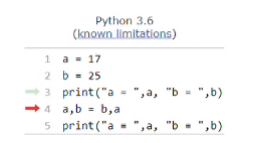
\includegraphics[width=0.5\textwidth]{./dados/figuras/cosso1.png}
    \fonte{Original}
    \label{fig:figura-mountPython}
\end{figure}

A tipagem fraca e o seu conteúdo ser dinamicamente tipada: o tipo de conteúdo de variável poder mudar automaticamente.

\begin{figure}[!htb]
    \centering
    \caption{Exemplo de Tipagem}
    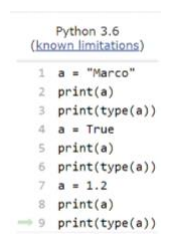
\includegraphics[width=0.35\textwidth]{./dados/figuras/cossin2.png}
    \fonte{Original}
    \label{fig:figura-mountPython}
\end{figure}

% Novo apêndice----------------------------------------------------------------
\chapter{Opinião: Iyan Lucas}
\label{chap:apendiceB}

Recentemente, comecei a exercer minha iniciação científica sob o Observatório da Saúde. 
Comecei a gostar de séries temporais e, apesar do meu apreço por linguagens como Java, C\# e C++, Python era essencial para tudo, desde a análise de dados à plotar pontos em mapas.
Fui, entre muitas áspas, "forçado" ao aprendizado da linguagem. 
Percebi de imediato, a minha estranheza com a falta de ponto-e-vírgula e chaves, sobretudo a ausência de uma main.
\par Agora, ao redigir este apêndice, estou bem acostumado ao Python, programando todo dia, todo meses com a linguagem e então me realizei da grandeza da LP.
Ela é, apesar de confusa, funcional, curta, simples e prática.
Fiquei assustado pela eficiência dela com grandes bases de dados e rapidez.
Apesar de que eu penso que faria os programas mais organizados e mais intuitivamente em Java, percebi que essa visão minha é só um ponto de vista de muitos.

\chapter{Opinião: Samir Cambraia}
\label{chap:apendiceB}

Depois da pesquisa, minha visão sobre a linguagem ficou mais abrangente.
Python é uma linguagem promissora com um grande currículo em aplicações em diversas áreas sendo a mais competente em em sua maioria, tendo sua simplicidade no aprendizado a programação possibilitando o conhecimento de rápida teoria/prática.
\par Porém, na minha opinião as estruturas e regras que levam a grande possibilidade de grandes códigos serem executados com menos trabalho e "linhas" é que me incomoda pelo fato de, como em java, se ter um controle maior e não esperar que a linguagem em si possibilite sem saber o que ocorre por trás assim pessoas com novas experiências, na minha opinião, ficaria rasas em conhecimento como na parte de memória e outros conhecimentos conquistados em linguagens de baixo nível que possibilitam maior controle.


\end{apendicesenv}
             			   % Apêndices
% \section{Anexo: Samir Cambraia}

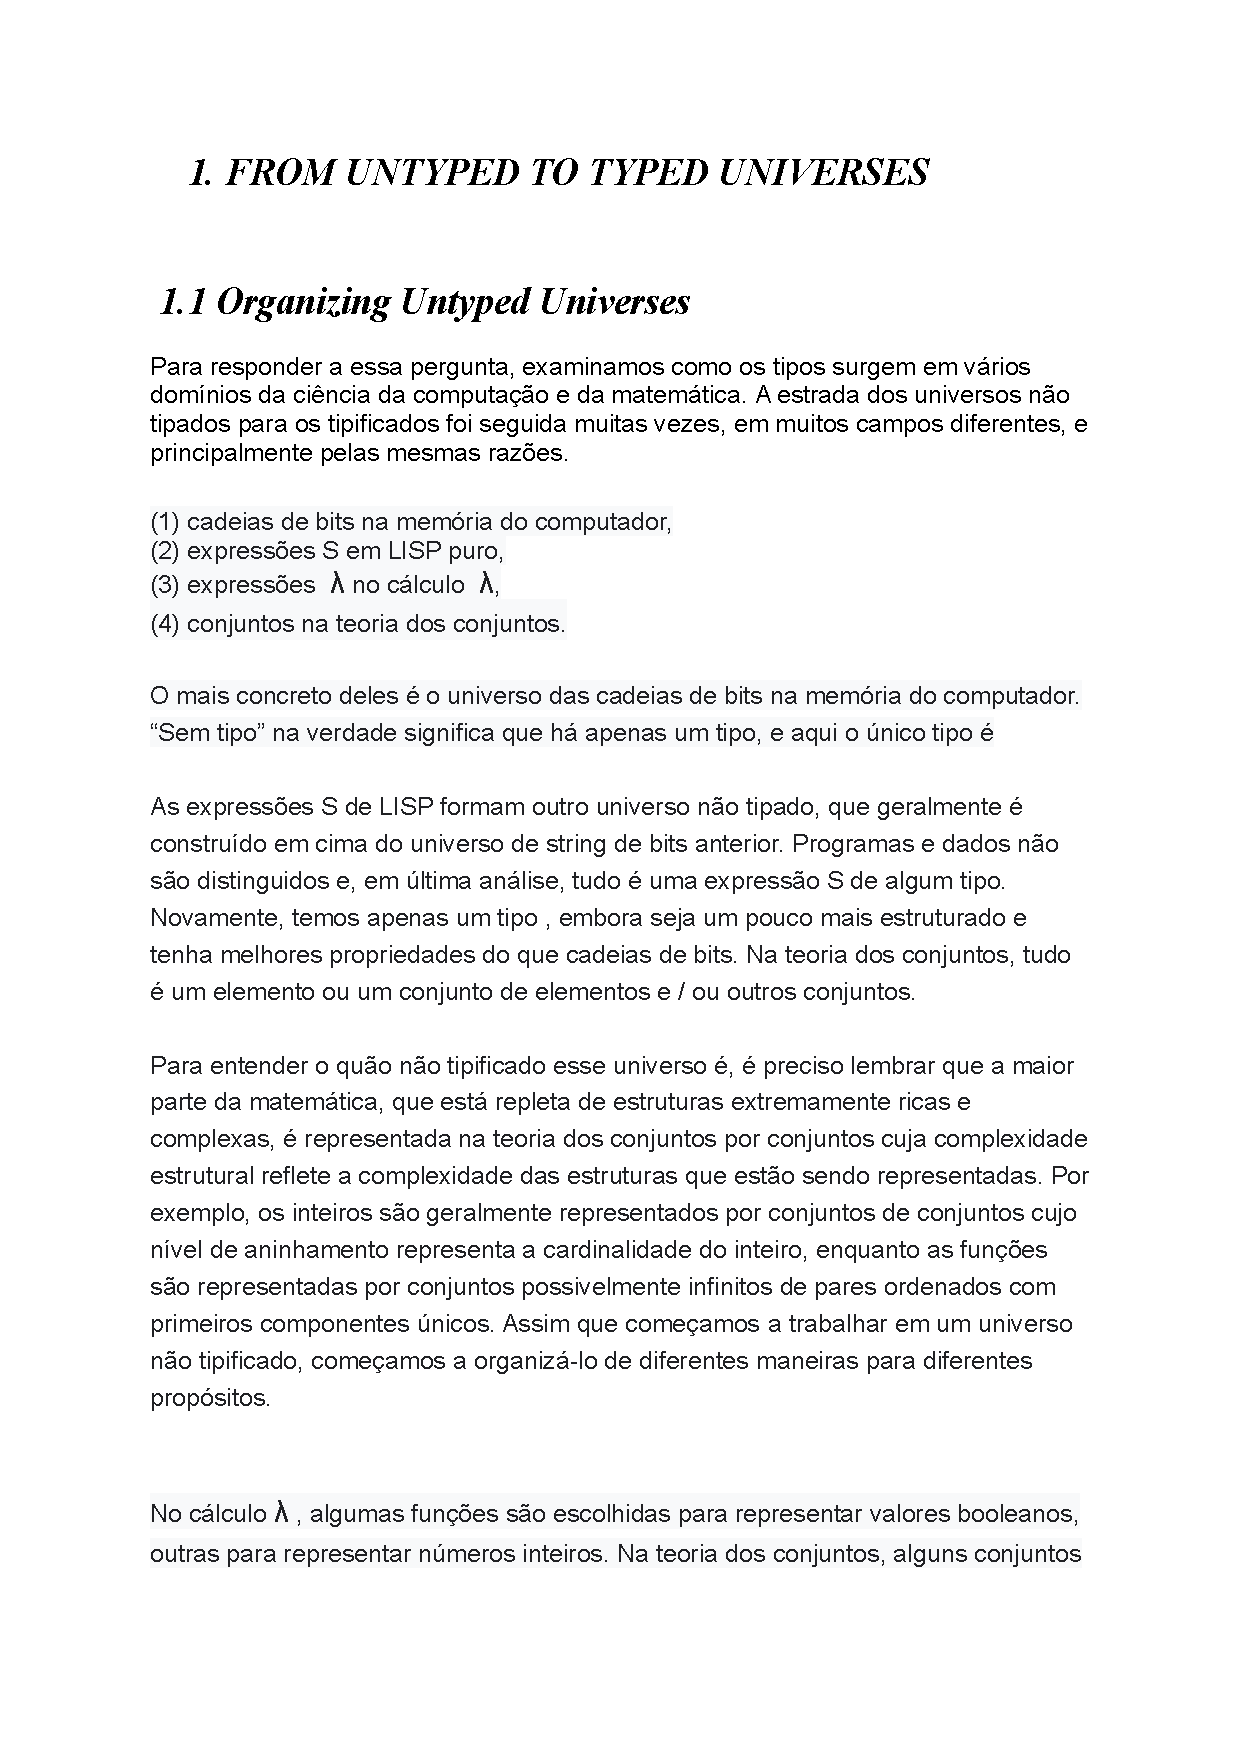
\includepdf[pages=-]{anexos/iyan.pdf}

\section{Anexo: Guilherme Cosso}

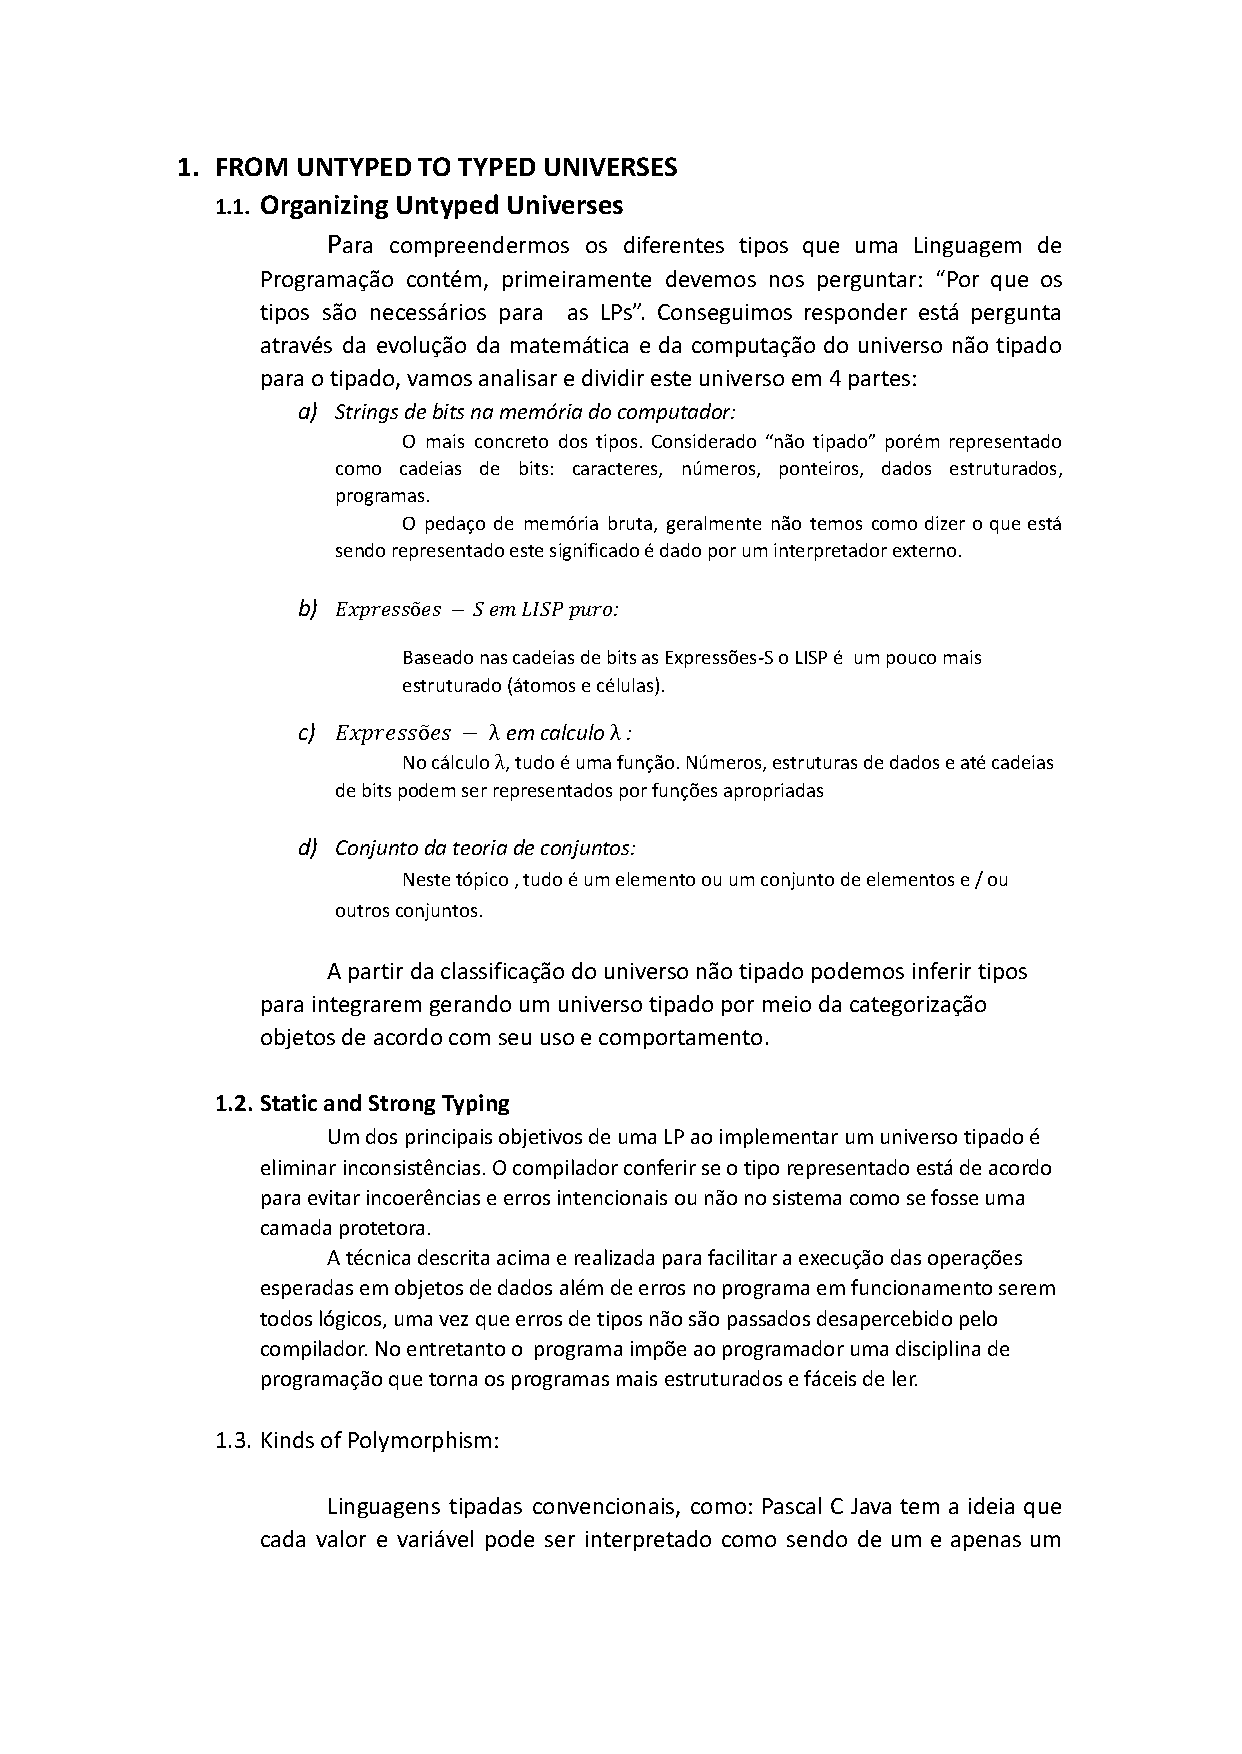
\includepdf[pages=-]{anexos/cosso.pdf}

\section{Anexo: Iyan Lucas}

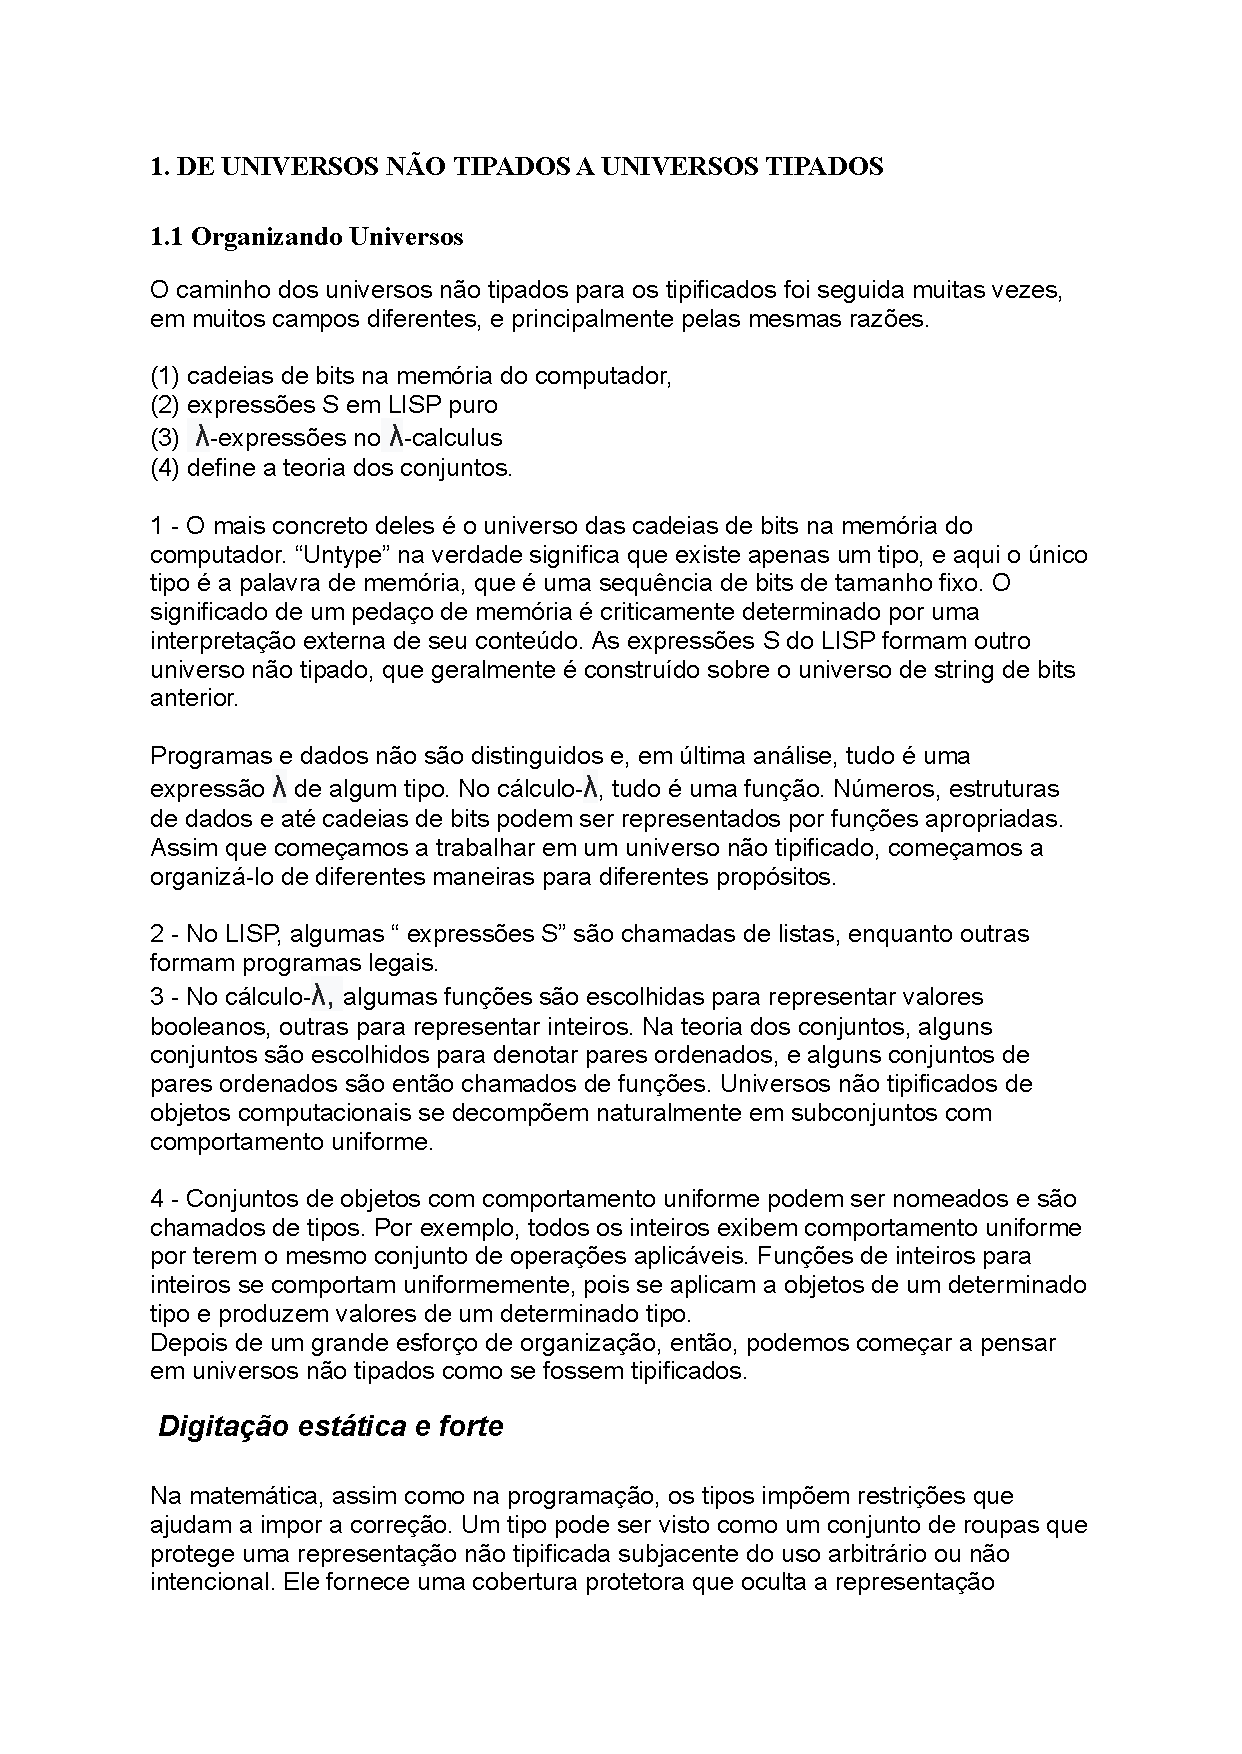
\includepdf[pages=-]{anexos/samir.pdf}
               			   % Anexos

\end{document}
